\documentclass[hyperref={pdfpagelabels=false}]{beamer}
\setbeamercolor{background canvas}{bg=white}
\usepackage{graphicx,lmodern,subfigure,ulem,color,graphicx,tikz,booktabs,natbib}
\usepackage{mathrsfs}
\usetheme{Warsaw}
%\definecolor{beamer@blendedblue}{rgb}{0.1,0.5,0.1}
%\definecolor{ForestGreen}{RGB}{60, 140, 60}
%\setbeamercolor{structure}{fg=beamer@blendedblue}
\setbeamertemplate{navigation symbols}{}
\setbeamertemplate{footline}[frame number]
\bibliographystyle{chicago}
\newcommand{\spitem}{\vspace{.3cm}\item}
\newcommand{\elas}{$E_{labor}$}
\def \ourFigPath {../../} 

\usetheme[
outer/progressbar=foot,
outer/numbering=none
]{metropolis}



\title{Project}
\author{Marco Brianti\\Vito Cormun}
\institute{Boston College}
\date{January 2019}


\begin{document}
	
	\frame{
		
		
		\maketitle
}



\frame{\frametitle{Sentiments Shocks and the Limit Cycle (I)}
	
In a series of recent papers Beaudry, Galizia, and Portier show that
	
	
	\begin{itemize}
		\item cycles are driven by economy's internal forces that favor cyclical outcomes
		
		
		\item and not by series of persistent positive and negative shocks
	\end{itemize}   
		
}

\frame{\frametitle{Sentiments Shocks and the Limit Cycle (II)}
	
	Their model with \textbf{stochastic limit cycle} strongly rejects the relevance of persistence shocks to explain the business cycles.
	
		\begin{itemize}
		\item cycles are driven by internal forces that favor a continuum of \textbf{boom-and-bust outcomes}
	\end{itemize}  
	
	\
	
	The role of disturbances is to deviate the expected trajectory of the cycle implying the unpredictability of its path.  
	
		
}

\frame{\frametitle{Our Contribution}
	
Does it mean that we should discard the plethora of models that generate mean reverting IRFs?

\


The answer is no. In particular, we show that
\begin{itemize}
	\item \textbf{Empirically}, cyclical patterns are only related to \textbf{sentiment shocks}
	\item \textbf{Theoretically}, we would like to rationalize this result with a model that displays
	\begin{itemize}
		\item boom-and-bust patterns to sentiment shocks
		\item mean reverting responses to technology, monetary and fiscal policies shocks
		\end{itemize}
	\end{itemize}
	
	
}
	

\frame{\frametitle{Econometric Procedure - Overview}
	
	We use a 2-step procedure
	
	\
	
	\begin{enumerate}
		\item Estimate series of sentiment shocks using forecast revisions of GDP growth at 4 quarters horizon
		
		\
		
		\item Estimate IRFs via local projection \`a la Jorda (2005)
	\end{enumerate}
	
}


\frame{\frametitle{Step 1 - Overview}
	
	We estimate sentiment shocks as SPF forecast revisions of real GDP growth rate which are orthogonal to 
	
	\
	
		\begin{enumerate}
		\item contemporaneous structural shocks
		
		\
		
		\item lagged principal components from a large dataset
		
		\
		
		\item past and future TFP
	\end{enumerate}
	
}


\frame{\frametitle{Step 1 - Estimation of $Z_t$}
	
	Data 
	\begin{itemize}
	 \item $X_t$ is log of Real GDP at time $t$
	 \item $X_{t+k|t} = E[X_{t+k}|I_t]$ provided by SPF
	 \end{itemize}
 
 \
 
 Procedure
	$$
	Z_t = (X_{t+4|t} - X_{t|t}) - (X_{t+4|t-1} - X_{t|t-1})
	$$
	where 
	\begin{itemize}
	\item $(X_{t+4|t} - X_{t|t})$ is expected growth rate of Real GDP conditional on information set up to time $t$
	\item $(X_{t+4|t-1} - X_{t|t-1})$ is expected growth rate of Real GDP conditional on information set up to time $t-1$
	\item $Z_t$ is an innovation to the expectations of output growth rate
	\end{itemize}
}


\frame{\frametitle{Step 1 - Estimation of $\tilde{Z}_t$}
	\textbf{Problem.} ${Z}_t$ is correlated with current and future fundamentals such as fiscal policy, monetary policy, current and future TFP.
	
	\
	
	\textbf{Solution.} Estimate $\tilde{Z}_t$ as the residual of the following regression,	
$$
Z_t = C +  \sum_{j=-J}^H \delta_j \Delta TFP_{t+j} + \gamma SS_t + \mu PC_{t-1} + \tilde{Z}_t
$$
where
\begin{itemize}
	\item $C$ is a constant parameter
	\item $\Delta TFP_t$ is first difference of utility-adjusted total factor productivity at time $t$
	\item $SS_t$ is a vector of structural shocks at time $t$ possibly estimated via narrative approach
	\item $PC_{t-1}$ is a vector of principal component at time $t-1$
\end{itemize}

\

$\tilde{Z}_t$ represents a change in expectations which is orthogonal to any source of fundamental fluctuations, i.e. a \textbf{noise shock}.
	
}



\frame{\frametitle{Step 2 - Estimation of IRFs to $\tilde{Z}_t$}
	Define $Y_t$ to be the BP-filtered log-transformation of an endogenous aggregate macroeconomic variable.
	
	\
	
	Using standard OLS techniques we estimate $H$ regressions	
	$$
	Y_{t+h} = \Theta_h^Y \tilde{Z}_t + \epsilon_{t+h}
	$$
	where $h = 1,2, \dots, H$ represent the forecast horizon.

	
	\
	
$\Theta_1^Y, \ \Theta_2^Y, \ \dots, \ \Theta_H^Y$ represent the path of the impulse response function of $Y_t$ to a unit deviation of $\tilde{Z}_t$.
	
}

\frame{\frametitle{Bootstrapping Techniques}
	
	\begin{enumerate}
		 

	
\item Consider the tuple $\Gamma^Y_h = \{ Y_{t+h}, \ T_t, \ \tilde{Z}_t, \ X_{t-1} \}$.

\

\item Divide $\Gamma^Y_h$ over time $t$ in smaller blocks and randomly reorder these blocks in order to form a new tuple $\Gamma^Y_{h,Boot1}$ of the same size of the previous one.

\


\item Estimate $\Theta_{h,Boot1}$ from $\Gamma^Y_{h,Boot1}$ using standards OLS techniques.

\

\item Redo (1)-(3) $2000$ times and select confidence intervals.

	\end{enumerate}	
	
}



\frame{\frametitle{Local Projection - Confidence Interval 68\% and 90\%}
	
	\begin{center}
		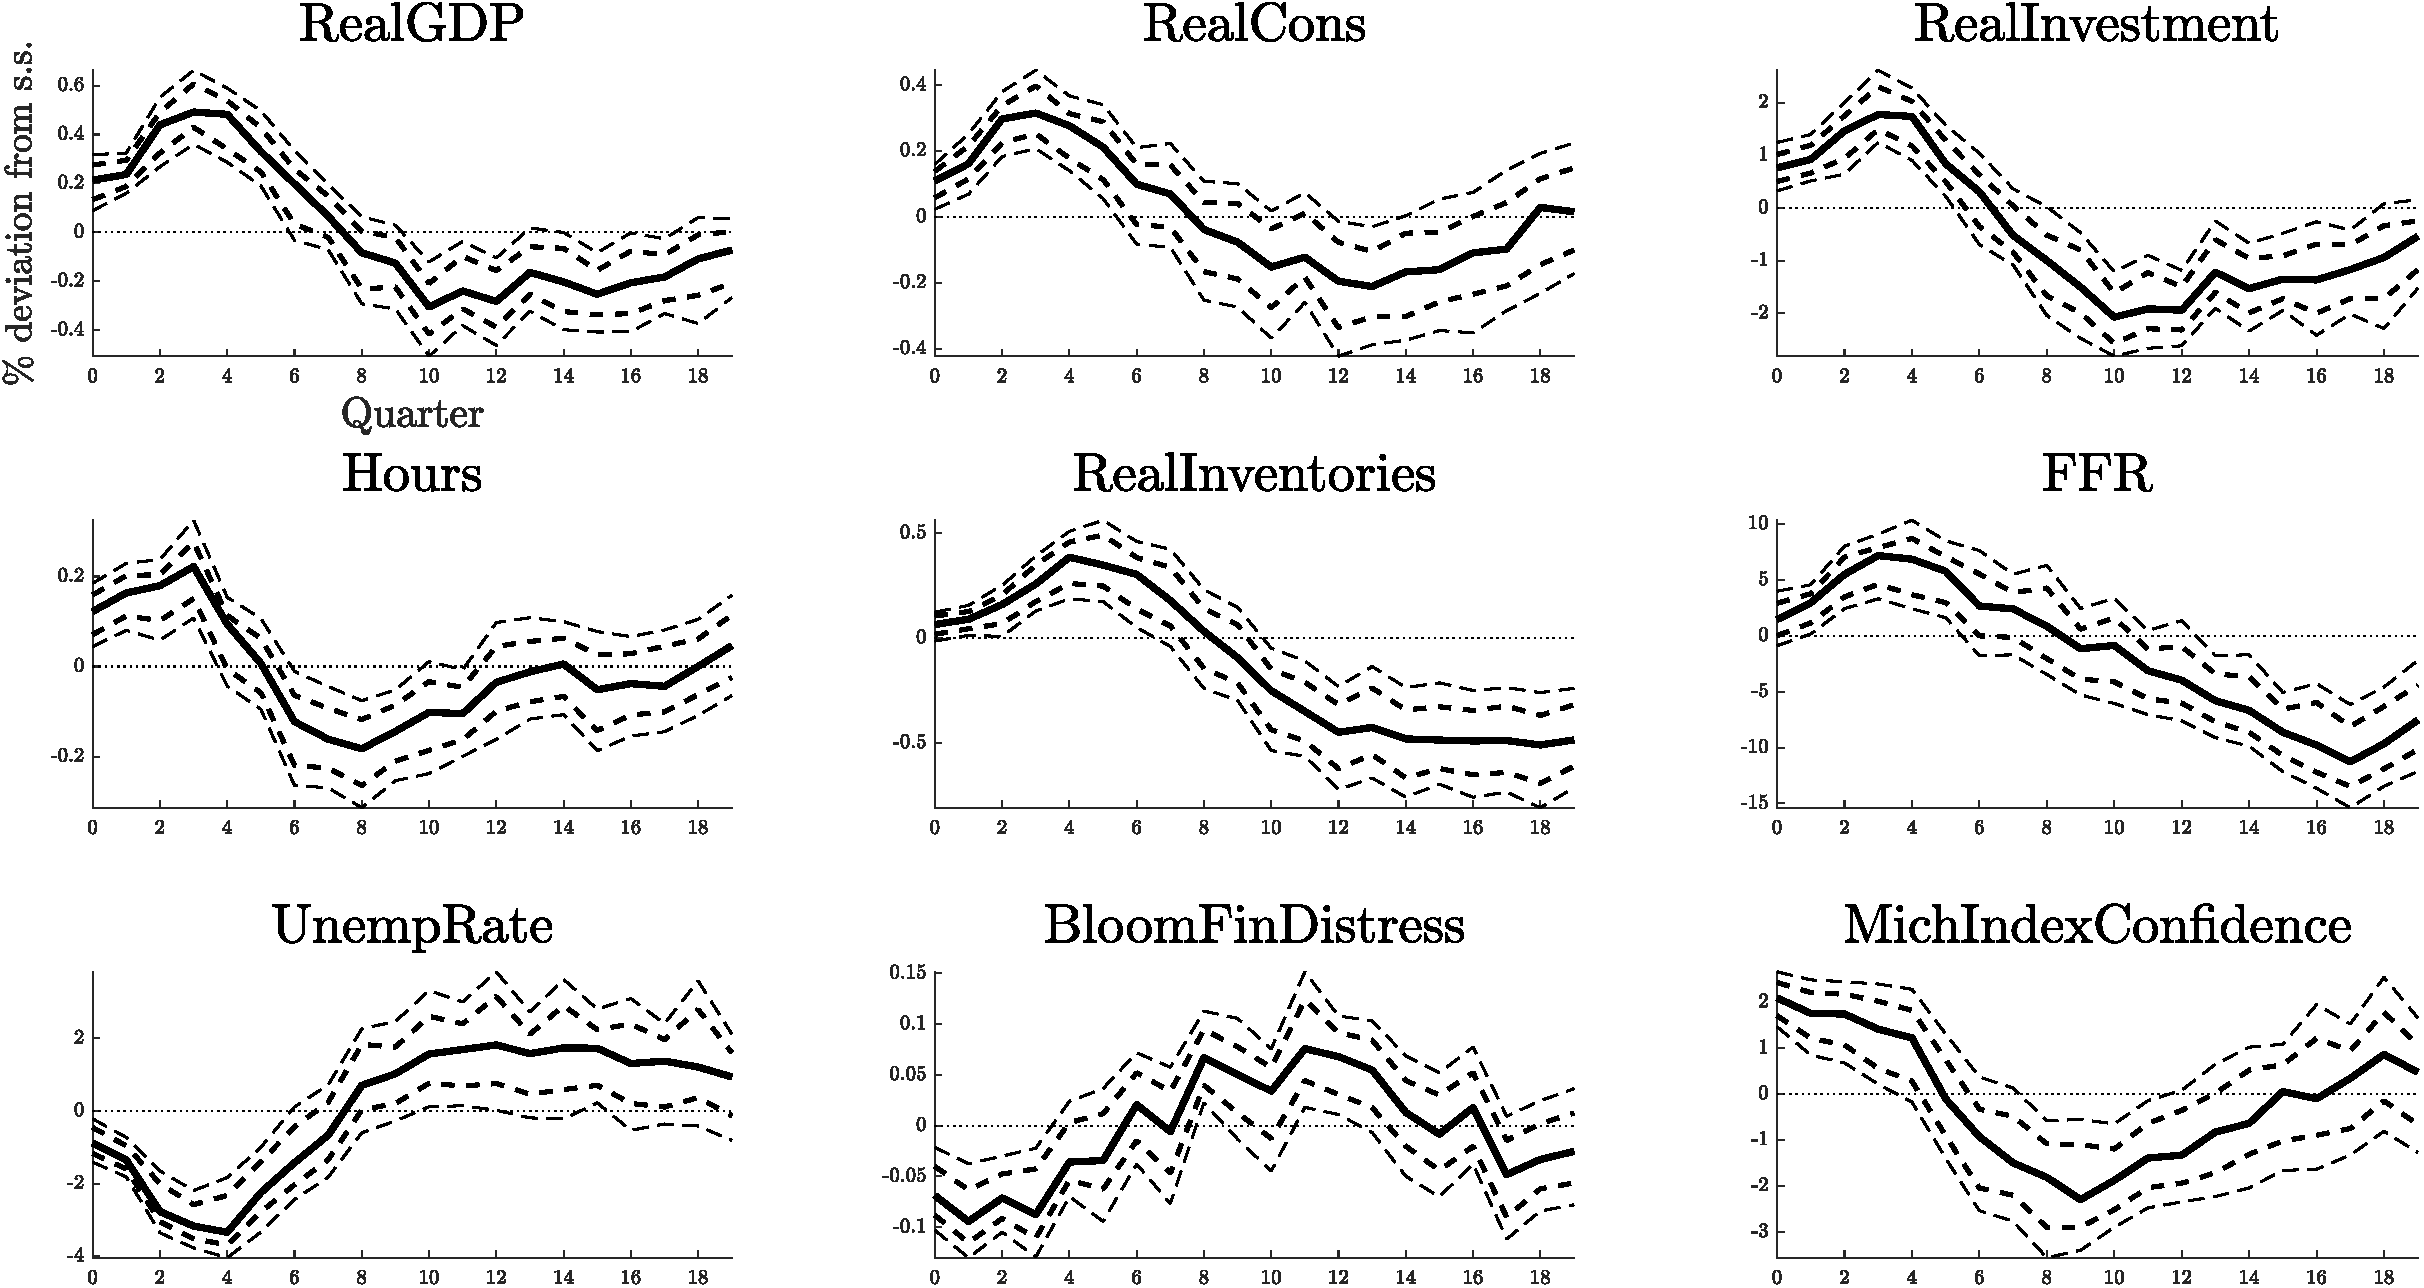
\includegraphics[scale = 0.27]{\ourFigPath Figures/ResInsideLP_20Dec2018}
	\end{center}
	
	
}



\frame{
	\frametitle{Testing the existence of cycles generated by structural shocks}
	Idea: given a structural shock a cycle emerges \textit{iff} the shock induces a local peak in the spectral density. \\
	
	\vskip 7pt
	
	Based on Canova (1996) and Beaudry Galizia Portier (2019) but applied conditioning on a shock \\
	$\hookrightarrow$ Unlike them we compute the spectrum parametrically using truncated IRFs.
	
	\vskip 10pt
	
	Under the null the shock generates a spectral density monotonically non decreasing in the periodicity \\
	$\hookrightarrow H_0:$  the IRF belongs to an AR(1) process with persistence of magnitude $\in [0,1)$.
}

\frame{
	\frametitle{Implementation}
	\begin{enumerate}
		\item Compute IRFs from data and bootstrap using Local Projections.
		\item Compute the spectrum as 
		$$y_t = B(L)\epsilon_t \Rightarrow S_y(\omega) = B(e^{-i\omega})S_\epsilon(\omega)B(e^{i\omega})$$
		Provided that the structural shock is a white noise, 
		$$S_y(\omega) = \frac{\sigma^2_\epsilon}{2\pi} B(e^{-i\omega})B(e^{i\omega})$$
		\item Define $D_1$ as the average spectral density over some window around 25 quarters, and $D_2$ the average around 60 quarters. The test statistic is $D = D_1/D_2$. 
		\item $H_0: D \leq 1$. Note that $D = 1$ under a white noise while it is smaller than one for an AR(1) with positive persistence.
		\item Compute p-value using bootstrap. 
	\end{enumerate}
}



\frame{
	\frametitle{Implications from findings}
	
	Results suggest a model where
	
	\begin{itemize}
		\item Sentiments are not correlated with TFP and policy shocks. Related, the model should not generate an invertibility issue.
		\item Sentiments generate boom-bust dynamics while fundamental shocks don't.
		\item Sentiments generate comovement in the real variables while they are non inflationary
		\item Sentiments explain only 12\% of stock prices while they explain almost 40\% of variations in real GDP
	\end{itemize}
}

\frame{
	\frametitle{Model?}
	What are sentiment shocks?
	\begin{itemize}
		\item Preference shocks, expectational errors, self-fullfilling fluctuations
	\end{itemize}
	\vskip 10pt
	How do we obtain boom and bust dynamics after a shock?
	\begin{itemize}
		\item In a unique equilibrium framework with imperfect info resulting in overaccumulation due to expectational errors$\rightarrow$ What are the information assumptions that we can make?
		\item Steady state is a sink $\rightarrow$ all shocks would generate boom and bust(?) (Benhabib and Farmer 1994)
		\item Multiple steady states and equilibrium is (locally) unique $\rightarrow$ economy is temporarily in the proximity of the bad steady state after a shock (Boissay Collard and Smets 2016)
	\end{itemize}
}
\frame{
	\frametitle{Questions raised}
	\begin{itemize}
		\item What's the meaning of boom and bust? Look at this IRF, does it display a peak?
		\item Cycle emerges \textit{iff} \dots is a definition or a result? A definition
		\item Doesn't the spectral density converges to zero by construction? No, because (?)
		\item Related, shouldn't the truncation horizon affect mostly the estimation of the spectral density at longer periodicities? No, it's the opposite, because (?)
		\item Why you do not search or compute the global maximum? Ok that you answer by saying that you follow the literature
		\item Ok that model with self-fullfilling shocks gives you the wrong movements in response to tfp shocks
		\item Try my model with Gaetano, sentiments shoould give you boom and bust while permanent tfp shocks should give you the right dynamics. 
		
	\end{itemize}
}
\frame{
	Rayan's view is that we could write a model in the spirit of Chahrour and Gaballo where after sentiment shocks the bust emerges because agents realize they were wrong. This implies that agents'information set is smaller than econometrician's info set. That agents do not know aggregate variables is consistent with Chahrour and Ulbricht.
	\vskip 10pt
	However, in CG agents learn from prices. But in our model prices decrease after the shock, which is not consistent with the idea of having an improvement in the local conditions, we need to think hard about how to get the right price movement.
}

\end{document}









\end{document}